\chapter{Introduction}
\label{c.intro}

The last decade has been revolutionary for computer architecture, and the next decade promises to be even more so.
While we have long had to adapt our design philosophies to account for changing physical constants,
fundamental relationships between technology properties have begun to drift from their comfortable trends.
We will no longer be able to rest on the twin laurels of Moore's Law and Dennard scaling to achieve the
expontential increases in computational performance that our information society has grown to depend upon.
As process scaling fails to produce further returns, architecture and design will have to take its place.

New design challenges call for the creation of new tools and the adoption of new methogologies.
Best practices for the hardware design industry have been complacently static.
In the meantime, software engineers have continued to push the boundaries of what is possible with the computers we have architected for their use.

This thesis is an attempt to apply the productivity of modern software tools to the design of future hardware architectures.
In extending the capabilities of a new hardware description language, I hope to have brought the agility and composability of functional, object-oriented software design to one of the most difficult design tasks in the hardware domain,
namely that of coherent hierarchies of on-chip caches.

This chapter provides an introduction to a current set of challenges facing the field of computer architecture.
I first discuss the genesis of modern hardware design objectives,
and then constrast those needs with the capabilities of modern design practices.
In doing so, I hope to illustrate the role my thesis plays in bringing the latter to bear on the former. 

\section{Landscape of Computer Architecture}

As I began my tenure at Berkeley, the computer processor industry was pivoting to adopt multicore chip designs,
in which multiple processors with a shared memory hierarchy are collated into a single chip.
This change was not perceived as welcome; the difficulties in achieving improved software performance that strongly scales with core count are substantial \cite{Asanovic:EECS-2006-183}.
Over the preceding decade, the processor industry had been backed into the multicore corner by three fundamental bottlenecks:
\begin{description}
\item[ILP Wall.] There are diminishing returns on automatically extracting more Instruction-Level Parallelism from sequential programs \cite{hennessy2011computer}.
\item[Memory Wall.] Memory latency improvement has been lagging memory bandwidth, and now even complex arithmetic operations are hundreds of times faster then loads and stores \cite{wulf1995hitting}.
\item[Power Wall.] We can put more transistors on a chip than we can dissipate the heat of switching at high frequency \cite{shacham-micro10}.
\end{description}

However, despite the ongoing dominance of multicore designs in the market, in the intervening years it has not proven to be pragmatic to for industry to exponentially increase core counts per chip alongside transistor counts.
Amdahl's law ensures that communication costs will eventually dominate any parallel program, so the marginal energy cost of increasing performance with parallelism increases with the number of cores.
Furthermore, parallelism itself does not intrinsically lower the energy per operation.
Faced with such diminishing returns, chip designers have instead looked to increasing the heterogeneity of the cores available on each chip, leading to the rise of System-On-a-Chip designs (SoCs) containing a variety of specialized cores.
The rest of this section provides context on how our industry got us where we are now, and where further technology scaling issues are likely to lead us.

\subsection{The End of Dennard Scaling and Moore's Law}

In 1965, Gordon Moore noted that the number of transistors than could economically be made to fit on an intergrated circuit had been doubling approximately every year and forecast that this trend would continue \cite{moore2006cramming}.
While he was making an empirical observation rather than stating a law of nature, history has proven his prediciton so accurate that the term ``Moore's Law'' is now synonymous with ceaseless technology scaling in a variety of contexts.

Robert Dennard in turn described how the transistor scaling predicted by Moore would translate into the device characteristics of metal-oxide semiconductor (MOS) devices \cite{dennard1974design}.
Dennard showed that when voltages are scaled along with all physical dimensions, a device's electric fields remain constant.
Therefore, most device characteristics are preserved with scaling, and specifically power usage remains proportionate to area.
This relationship enabled chip designers to pursue several decades of aggressive, high-frequency designs based on assumptions of unconstrained power consumption.

Unfortunately, in the last decade Dennard scaling has broken down.
As voltages have dropped, exponentially increasing static leakage power losses take up an ever greater proportion of the overall power supplied.
Leakage losses heat up the chip, which further exacerbates static power loss and raises the spectre of thermal runaway.
Fear of leakage has thereby halted voltage scaling, leading to dramatic increases in power density as we continue to try to increase the average number of gate switches per second. 
While this power wall has already spurred industry towards multicore designs, some forecasts predict a rapidly approaching era of ``dark silicon,'' where significant fractions of a chip must be power-gated off at any given time \cite{esmaeilzadeh2011dark}.

Ironically, we may yet be saved from a future of dark silicon by the fact that Moore's Law itself seems to be beginning to falter.
In July 2015, Intel announced that their next generation of processors will not be ready until 2017,
and that a third iteration on the design of the current processor generation would be used to fill in the gap.
This scheduling change pushed the cadence of their technology node jumps out to nearly three years,
and also broke the ``tick/tock'' model of design-change-or-technology-shrink per generation that the company had been holding fast to since 2007.
The proximal effect of the slowdown is for Intel and other companies to increase the number of design iterations they cycle through at each technology node.
In order to add value to the next product, companies will have to improve the design while working with the same number of transistor resources.

Taken together, the rise of power constraints and limited transistor counts puts the emphasis of the computer processor industry back on chip design and architecture, rather than process technology scaling.

\subsection{Designing for Energy Efficiency}

In this brave new power-constrained, post-Dennard world, energy efficiency becomes a first-order design goal.
Power is the product of performance (operations per second) and energy per operation.
Therefore, subject to power constraints, the only way in which hardware designers can continue to offer increasing performance is to lower energy per operation.
Energy efficiency demands for high-performance computing and embedded computing have converged due to the former's hunger for maximal performance and the latter's dependence on battery life.

Providing specialized hardware is a natural solution to reducing energy per operation while also playing nicely with the dark silicon paradigm \cite{esmaeilzadeh2011dark}.
For a particular problem, some subset of the transistors can be used to arrive at a solution as efficiently as possible, while less suitable portions of the chip remain power-gated.
This trend has already become manifest in the embedded and mobile device industry via the adoption of SoC designs, which boast an ever increasing number of specialized co-processors on each chip.
These specialized units handle applications as diverse as voice recognition, audiovisual codec playback, image stabilization, radio and WiFi signal processing, and many more.
The reseach community has also begun to study frameworks for exploring design spaces of extremely heterogenous designs.
Some researchers have advocated building chip generators that can be retargeted for application-specific needs \cite{shacham-micro10}.
Others have focused on creating seas of specialized units from High-Level Synthesis tools \cite{shao2014aladdin, Venkatesh:2010}.

Moving beyond specialized cores, energy consumption within the memory hierarchy is rapidly becoming a significant design concern.
The trend can be seen most clearly by contrasting the energy costs of performing arithmetic operations with the costs of transporting the operands to the unit which will carry out the computation.
Table~\ref{tab:movement} presents an overview of the relative costs of computation versus communication in a 45nm process \cite{dally-hpca02}.

\begin{table}[tdp]
\begin{center}
\begin{tabular}{|c|c|} 
\hline
Task & Energy (pJ) \\ \hline
32B ALU Op & 0.3 \\ \hline
32B read from register & 0.6 \\ \hline
32B read from 8KB SRAM & 3 \\ \hline
32B transfer across chip & 17 \\ \hline
32B read from off-chip DRAM & 400 \\ \hline
\end{tabular}
\end{center}
\caption{Energy costs of computation versus communication in 45nm \cite{dally-hpca02}. }
\label{tab:movement}
\end{table}

As is clear from these estimates, data movement energy costs far outweigh the computation's energy costs, even for simple reads of local register files.
Transferring data across the entire chip is yet more expensive.
The high cost associated with communication thereby increases the value of managing the memory hierarchy well.
Ineffective heuristics for data placement and replication within the on-chip memory hierarchy can potentially waste a vast amount of energy relative to the base cost of the computation itself.

In a multicore chip with a signficant hierarchy of on-chip caches, the majority of the data movement activity that occurs within the chip is done automatically at the behest of the cache controllers and the coherence policy that governs their behaviors.
Since traditional cache coherence protocols preserve the abstraction of a global memory shared by all the cores,
they must work behind the scenes to keep copies of data in the right places,
potentially trading off additional communication for improved performance.
How to define customizable coherence policies, implement the associated protocols efficiently,
and manage the aforementioned communication/performance tradeoff is an important design challenge for future energy-efficient architectures. 

\subsection{The Future of Cache Coherence}

Modern multicore processors communicate by executing load and store instructions that reference a shared global address space, or {\em shared memory}.
However, the cores also make use of hardware-managed caches to reduce the expected latency of these memory requests, as well as to filter outbound memory traffic.
Generally these caches are organized into a tree, where the root is a large shared cache and the leaves are private caches co-located with each core.
Because the levels of the memory hierarchy closest to the cores are private, hardware mechanisms must be provided by the chip designer to ensure that all caches agree on the value stored at each memory address at a given point in time.
This agreement is what makes the system {\em coherent}.

In a system with hardware-managed cache coherence, the cache controllers and memory controllers
communicate among themselves according to some protocol to maintain coherence.
While they might have vastly different implementations, 
all such protocols maintain coherence by ensuring the same {\em single-writer, multiple-reader} (SWMR) invariant \cite{sorin2011primer}. 
For a given block of cached memory, at any given moment in time, there is either: 
(1) a single core that may write (or read) the block, or 
(2) there are zero or more cores that may read the block.
Violating this invariant could lead to values stored out by one core never becoming visible to other cores.

The cache-coherent shared memory paradigm has dominated the multicore marketplace, from servers to mobile devices,
for both technical and legacy reasons.
In many cases, hardware-management of cache coherence provides performance that is superior
to that of software-managed solutions, while vastly reducing programmer effort \cite{leverich-isca07}.
At the same time, hardware-management innately provides backwards compatibility for operating systems and user-level software that has been written in the shared memory paradigm.

Despite its innate appeal, the future scalability of hardware-managed coherence has been a debated topic.
As core counts continue to grow, some researchers fear forthcoming increases in coherence-related traffic, coherence metadata storage overhead, and the maintainance of inclusive caches will dominate the performance benefits of hardware-managed coherence \cite{choi2011denovo, kelm2011cohesion, howard201048}.
Others have argued that backwards compatibility/legacy is too important to give up and that scalability challenges can be addressed \cite{martin2012chip}.

The scalability issue is somewhat mitigated by the fact that industry has shied away from exponentially increasing core count per chip, and instead moved to focus on specialization and heterogenous cores.
It seems probable that we will observe a continued inclusion of hardware-managed cache coherence, albeit possibly alongside software-managed solutions.
As the energy consumed by data movement continues to grow relative to that required to perform computations, more design effort will be put into optimizations for purely hardware-based protocols,
or into protocols that support optional software control of coherence for certain memory regions \cite{kelm2011cohesion}.

In general, we will see protocols that have been extended in order to reduce the average energy consumed in transferring the data required by particular accelerators or application-specific co-processors to the proper place and in the ideal layout.
This increase in complexity means that protocol design and verification will grow more both difficult and more important,
which is unfortunate because correctly implementing cache coherence protocols is one of the hardest tasks in hardware design.

\subsection{Correctly Implementing Cache Coherence Protocols}

Designing new cache coherence protocols or supporting a wider variety of more complicated protcols is not a task hardware engineers can undertake lightly.
Verifying the correctness of a cache coherence protocol is a challenging task, and
verifying that a correct protocol has been implemented correctly (using simulations or silicon) is even more difficult
\cite{deorio2008post, bentley2001validating, burckhardt2005verifying, clarke1995verification, dill1992protocol, wood1990verifying}.
Traditionally, protocol correctness is verified using an abstracted version of the distributed system of caches upon which the protocol operates
\cite{talupur2008going, delzanno2003constraint, pong1997verification, wood1990verifying, mcmillan2001parameterized}.
The abstraction employed at this stage makes the verificaiton process tractable by eliding many details of the underlying modules' implementations.
Upon verification of protocol correctness, hardware designers must then use a hardware description language (HDL) to write cache controller logic that correctly implements the protocol.

Unfortuntaely, the semantic gap between high-level abstract descriptions of protocols and 
concrete HDL implementations of those same protocols is so wide that verifying the correctness of the protocol
does not come close to guaranteeing the correctness of the final implementation \cite{dave-memocode05}.
There are a huge number of ways that details of the implementation can interfere with the behavior of the coherence protocol.
Hardware designers must work from scratch to manually maintain the implicit semantics of the abstracted protocol model in the controllers and networks they build.
Many modules designed by different teams must interact in the expected ways.
State machines must be correctly transliterated from the protocol's specification, possibly by hand.

As we will see, improving the capabilities of HDLs offers us a path foward to lighten this design burden.
By raising the level of abstraction at which cache controller logic can be described and at which synthesizable designs can be generated,
we can smooth over the gap between protocol specification and implementation.
In doing so, we can make cache coherence protocol selection another knob in the toolbox of a hardware designer focused on exploring a space of heterogenous hardware designs.

\section{Productivity in Hardware Design}

In this new world of energy-efficient, heterogeneous, application-specific designs, it will be essential to both improve the productivity of hardware designers as well as enable extensive design-space exploration of alternative system microarchitectures \cite{shacham-micro10}.
On the productivity side, we hope to take lessons learned from the software world and apply them to hardware design tasks.
On the design space exploration side, we need to expand the capabilities of hardware development tools and make our hardware development methodology more iterative.
For example, we hope that by introducing language constructs that support metaprogramming, 
we can allow developers to write design generators, rather than instances of designs,
which in turn will encourage them to develop their designs more iteratively while
incorporating design space exploration between each step.
This section provides context for what we hope to accomplish by mining the software development community's best practices in both language and methodology areas.

\subsection{The role of language}

Today's dominant hardware-description languages (HDLs), Verilog and VHDL, were originally developed as hardware simulation languages,
and were only later adopted as a basis for hardware synthesis \cite{palnitkar2003verilog}.
Because the semantics of these languages are primarily focused on describing extensible simulation environments,
synthesizable designs must be inferred from a particular subset of the language, complicating tool development and designer education. 
These languages also lack many powerful abstraction facilities present in modern software languages.
For example, only in the last decade has SystemVerilog introduced object-oriented concepts as basic as C-style structs to the hardware synthesis domain \cite{sutherland2006systemverilog}.
Limited abstraction capabilities lower designer productivity by making it difficult to reuse code by building up libraries of components.

To work around these limitations, one common approach is to use another language as a macro-processing language to stich together leaf components expressed in a traditional HDL. 
This philosophy reflects a bottom-up approach, where frameworks are created to wire together and abstract simple components, improving the productivity of humans exploring the design space.
For example, Genesis2 \cite{genesis2} uses Perl to provide more flexible parameterization and elaboration of hardware blocks written in SystemVerilog.
%Verischemelog \cite{jennings1999verischemelog} provides a Scheme syntax for specifying modules in a similar format to Verilog. 
%JHDL \cite{bellows1998jhdl} equates Java classes with modules. 
%HML \cite{li200hml} uses ML functions to wire together a circuit.
Unfortunately, these multi-language approaches to bottom-up design are cumbersome, as they combine the poor abstraction facilities of the underlying HDL with a completely different high-level programming model that knows nothing about the semantics of hardware construction.

An alternative approach is to express the design in terms of a domain-specific application programming language from which hardware blocks can be synthesized.
This approach is generally termed High-Level Synthesis (HLS) \cite{gajski2012hls}.
The HLS philosophy reflects a top-down approach, in which designers describe the intent or behavior of the design, and automated tools derive acceptable implementations.
%For example, Esterel \cite{berry1992esterel} uses event-based statements to program hardware for reactive systems.
%DIL \cite{budiu1999fast} is an intermediate language targeted at stream processing and hardware virtualization. 
%Bluespec \cite{bluespec} supports a relatively general concurrent computation model based on guarded atomic actions.
While HLS can improve designer productivity when the pattern encoded in the high-level programming model is a good match for the purpose of the hardware block being designed, it can be a struggle for designers to express tasks outside the domain of the high-level language.
Expanding the scope of tasks describable by a particular high-level language is difficult, and
in general the broader the high-level language is, the more difficult it becomes for the tools to derive an efficient microarchitecture.
The lack of direct control over the amount of hardware resources generated by the synthesis process also concerns some designers.

As described later in this thesis, we have pursued a syncretic language approach that allows for collections of components to be built up into reusable libraries, while also providing a substrate upon which HLS tools can be built.
By leveraging first-order language support for object-orientation and metaprogramming, 
our goal is to allow developers to write design generators rather than individual instances of designs,
which in turn will encourage them to develop families of customizable designs in new ways.
By embedding implicit microarchitectural and domain knowledge along with explicit evaluation data in the generators we construct, we can iteratively create different chip instances customized for particular design goals or constraints \cite{shacham-micro10}.
As constructing hardware generators rather than creating hardware designs requires
support for reconfiguring individual components based on the context in which they are deployed,
our new language also improves on the limited module parameterization facilities of traditional HDLs.

\subsection{The role of the development model}

\begin{figure}[t!]
\centering
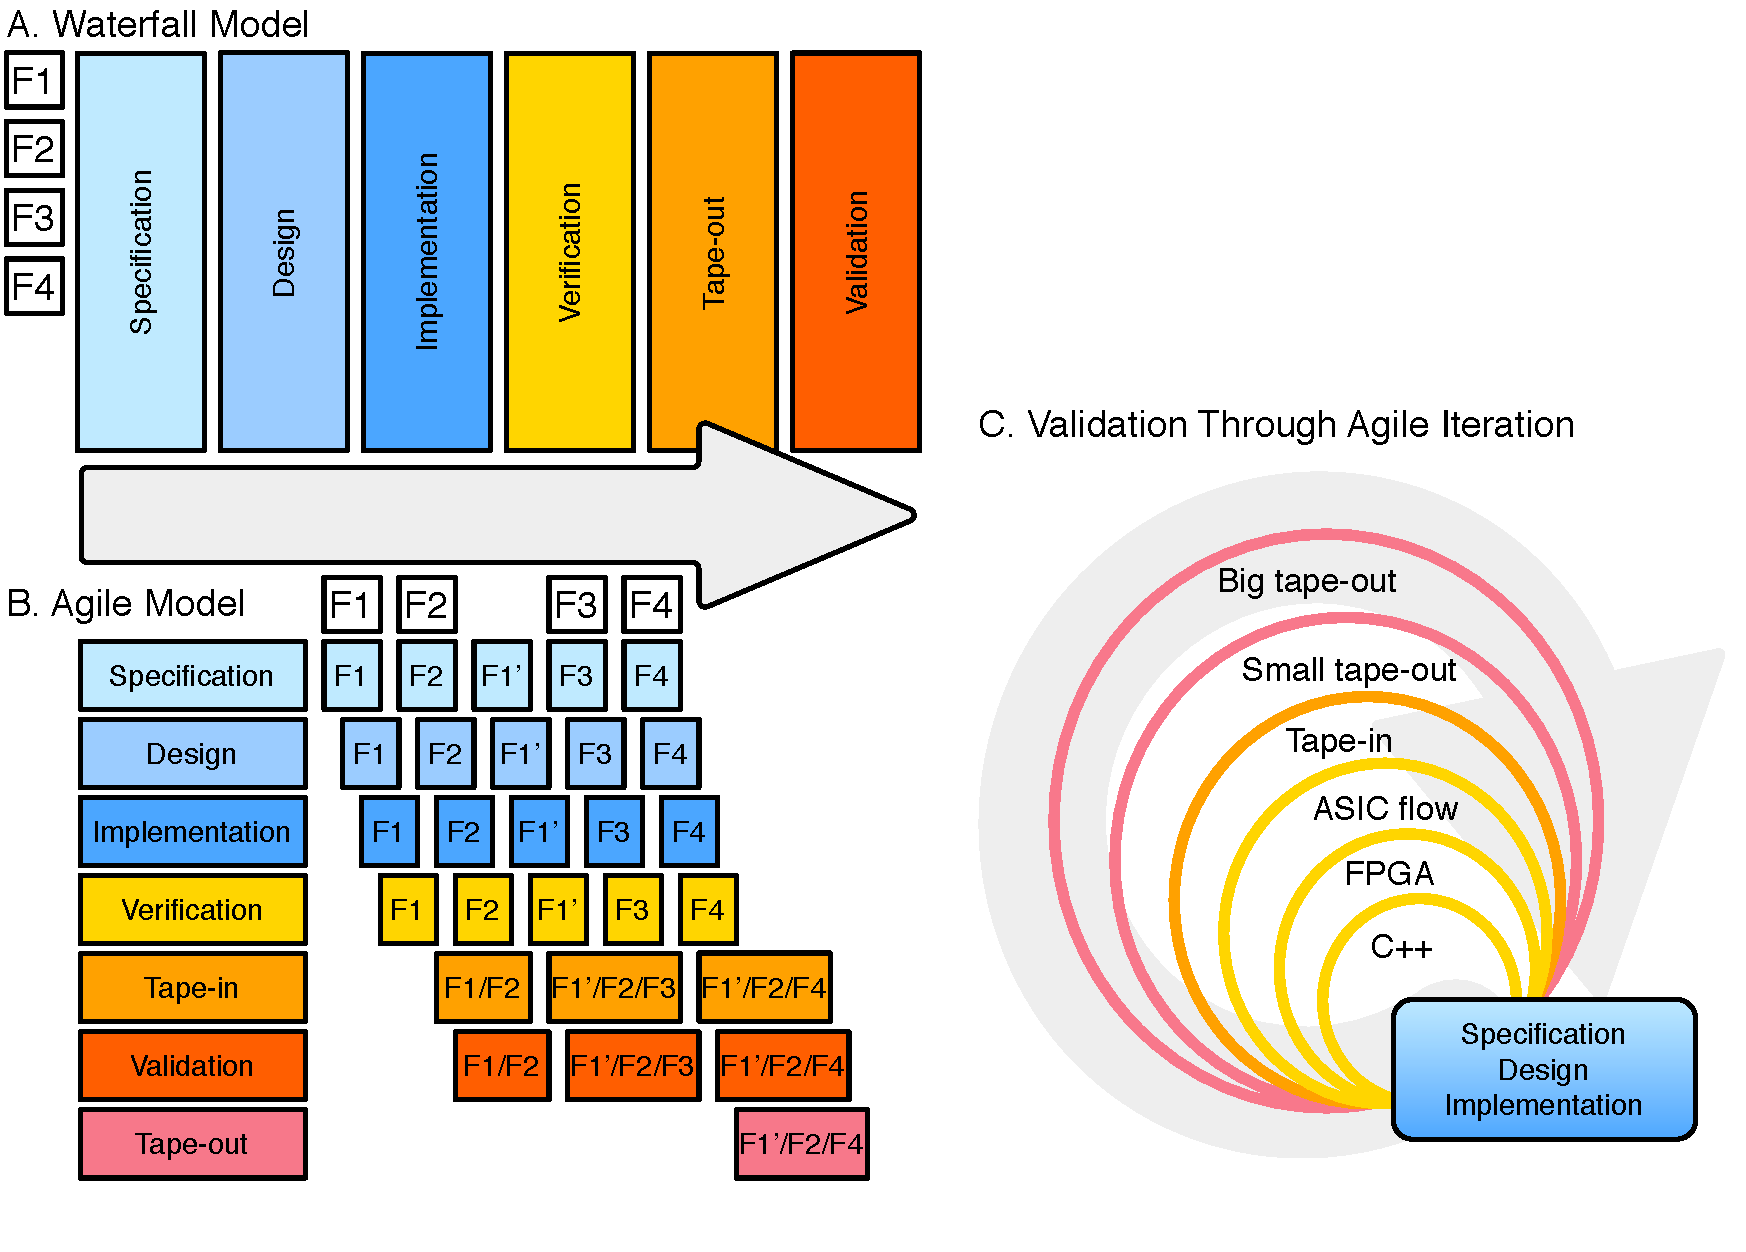
\includegraphics[width=1\columnwidth]{intro/figures/agile.pdf}
\caption{
A. The waterfall model steps all features through each activity sequentially.
B. The agile modle pushes each feature through all activities in parallel.
C. As we validate many features in parallel we push them through lengthier yet more accurate evaluation methodologies.
}
\label{fig:agile}
\end{figure}

Traditionally, both software and hardware have been developed as a sequential process that consists of distinct phases:
requirements analysis and specification,
architectural design,
implementation and integration,
verification and test,
operation and maintenance.
This process is the called the Waterfall development model, since it flows inexorably from the start of the project down through all phases until completion. 
Once a step has been completed, developers cannot return to a previous one without scrapping the whole project and beginning anew.
The Waterfall model relies on extensive documentation, meiticulous record keeping, and fixed client requirements.

The frequentcy of over-budget, late, and abandoned software projects led to a revolution in software development, demarcated by the Agile Manifesto in 2001 \cite{agile}.
Agile development methodology emphasizes interpersonal interactions over processes, working software over comprehensive documentation, and responding to change over following a plan.
Given a fixed time and cost, an agile team will create feature estimates, whereas a waterfall-based team will use a fixed plan to create time and cost estimates. 
In practice, the agile approach leads to small teams refining a set of working-but-incomplete prototypes iteratively until the end result is acceptable.
Decisions about what design elements to change in each future iteration depend on an evaluation of the previous one.
Rewrites and changes to requirements are to be expected, and in fact are forged into a competitive advantage for the client.

Figure~\ref{fig:agile} illustrates the agile development model in contrast to the waterfall model.
In our agile methodology, we first push a trivial prototype with a minimal working feature set all the way through the toolflow.
Then we begin adding features to it iteratively.  After spec'ing out a particular feature and implementing it, 
we then deploy it against an increasing series of more complex tests on more heavyweight evaluation platforms, up to and including taping out prototype chips.
Emphasizing a sequence of prototypes reduces verification simulation effort since early hardware prototypes run orders of magnitude faster than simulators. 

While there are some benefits in terms of verification (``are we building the thing right''), 
where the agile model really shines is validation (``are building the right thing''),
in that we are more likely to meet energy-performance expectations using the iterative agile process.
Figure~\ref{fig:agile}.C illustrates how we use the agile model to improve validation.
The circumfrence of each circle represents the relative time it takes to validate the design using a particular technology to achieve an ever increasing level of confidence.
While the latency and cost of these validation efforts go up, at the same time our confidence in verification and validation of the set of new features go up too.
Iterating in parallel at different levels of abstraction is the key to our productivity gains.
Feedback from previous iterations is used to drive the set of features emphasized in the next round of development.

Conventional wisdom holds that the frequent deliverable prototypes required by agile methodology are incompatible with hardware development, but our research group has not found this to be the case \cite{lee-micro15}.
While mask costs for modern designs are on the order of multiples of millions of dollars depending on process technology \cite{sperling}, 
organizations like MOSIS continue to offer multi-project wafers, where many independent projects are put on the same reticle, to help amortize these mask costs.
By reducing the minimal die size to around 1.5x1.5 mm we were able to bring the total cost of our prototype chips down to \$30,000,
and produced eleven chips over the course of just four years with a small team of graduate students.
It is worth noting that three distinct families of chips were produced in an interleaved fashion, {\em all from the same source code base}, but specialized differently to try out distinct research ideas
(see Figure~\ref{fig:tapeouts}).
As Moore's Law continues to slow down, industry will spend more time on each process technology node, leading to further reductions in the cost of doing multiple design iterations at a given node.

While the four-month latency inherent to the fabrication and evaluation of test chips may seem ponderous to agile software developers,
it still allows for three to ten times as many iterations compared to the traditional  multi-year turnaround of large chip designs flowed painstakingly through the waterfall model.
By supplementing the actual external test chip tapeouts with internal evaluations of further prototypical iterations, we can further reduce our team's iteration latency.
This approach also encourages reuse of a shared software stack and verification framework, further amortizing costs.

Adopting the agile methodology dovetails nicely with our emphasis on building chip generators over particular chip design instances.
As we add features to the generator, we can retarget our efforts to adapt to performance and energy feedback from the previous iteration.
By parameterizing the design, we can scale it from test chip sizes to final product without rewriting any modules.
As we will see, even a design choice as complicated and pervasive as a multi-level cache coherence protocol can be made a tuneable design parameter when properly factored out from the rest of the design.
By providing support for generating a family of protocols rather than one single protocol, my thesis has enabled us to iterate on protocol design as we scale up the size of the memory hierarchy across chip iterations.

\begin{figure}[t!]
\centering
\vspace{-0.15in}
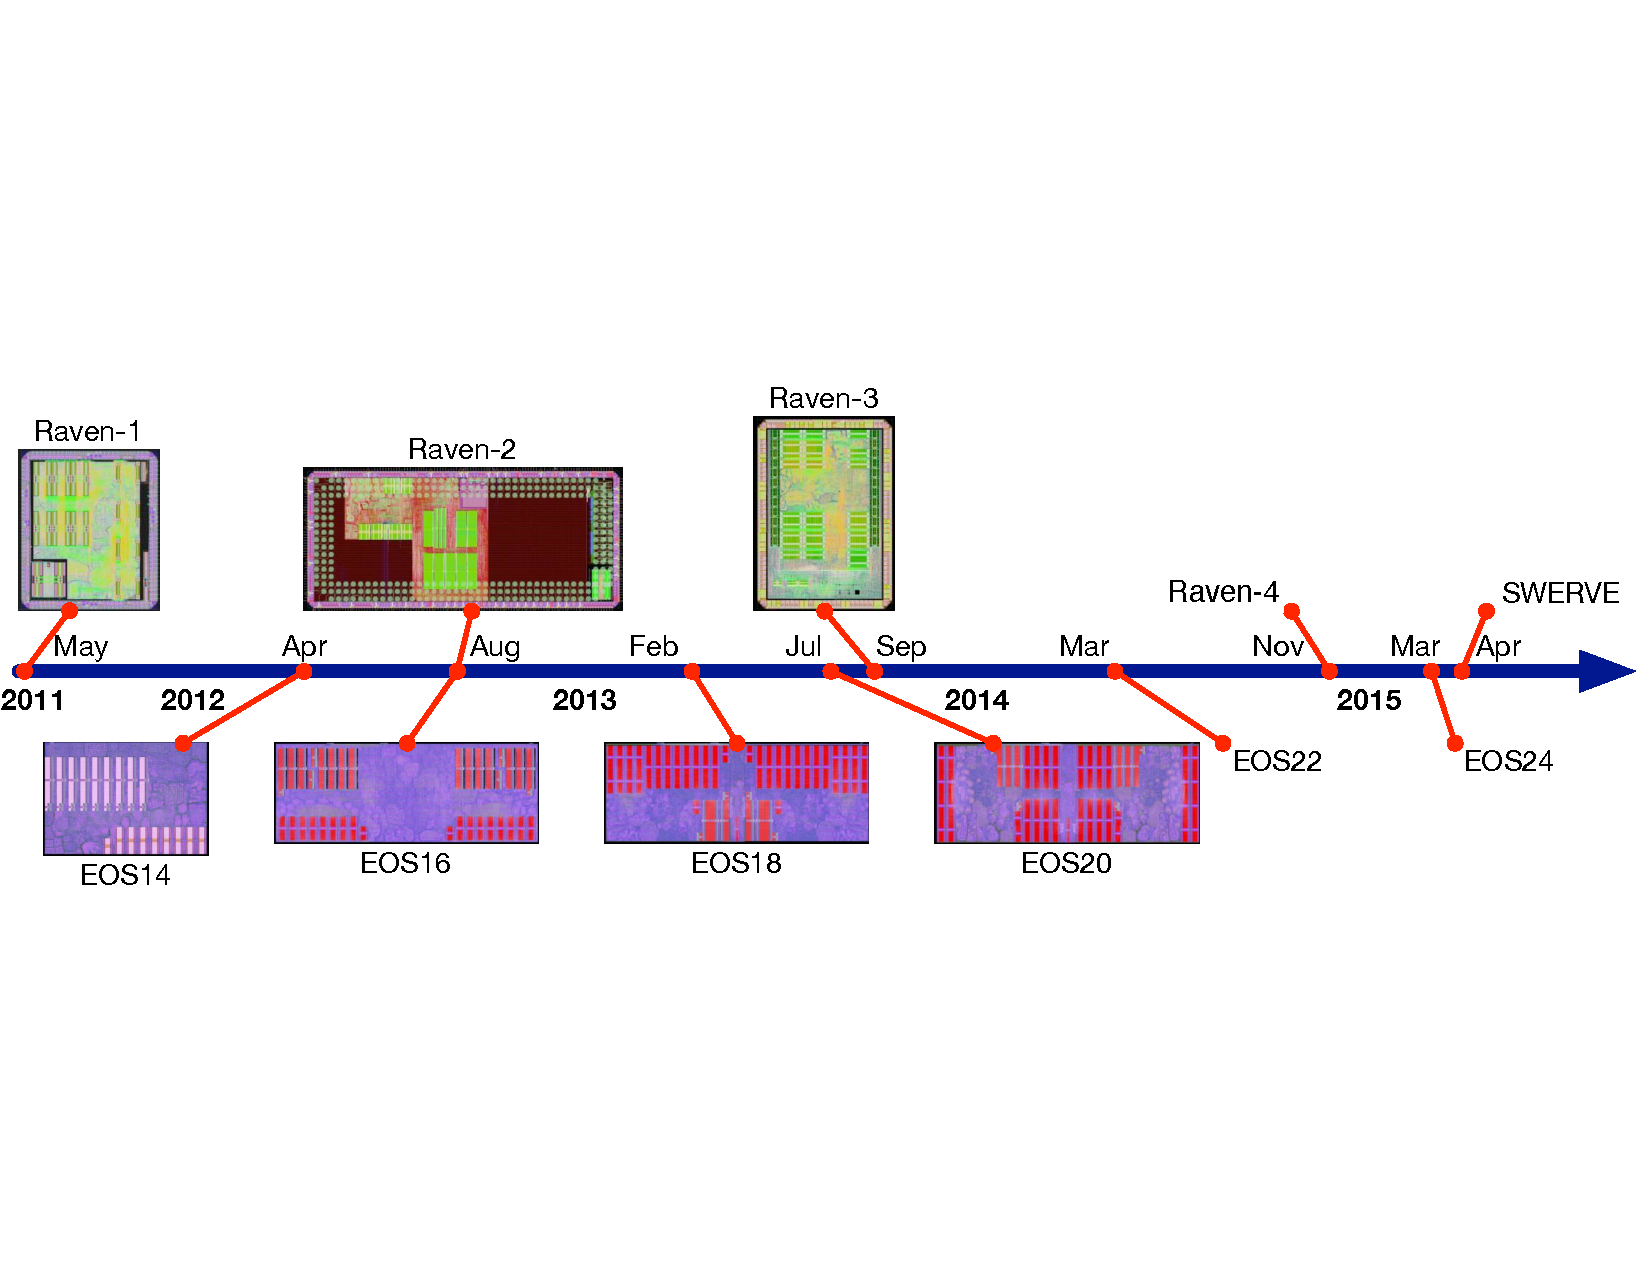
\includegraphics[width=\columnwidth]{intro/figures/tapeouts.pdf}
\vspace{-0.3in}
\caption{Lineage of UC Berkeley Chip Tape-Outs during the completion of my thesis.
The 28nm Raven chips combines a 64-bit RISC-V vector microprocessor with on-chip switched-capacitor DC-DC converters and adaptive clocking ~\cite{zimmer2015raven}.
The 45nm EOS chips integrate a 64-bit dual-core RISC-V vector processor with monolithically-integrated silicon photonic links ~\cite{lee2014eos}.
In total, we have taped out
four Raven chips on STMicroelectronics' 28nm FD-SOI process,
six EOS chips on IBM's 45nm SOI process,
and one SWERVE chip on TSMC's 28nm process. 
}
\label{fig:tapeouts}
\vspace{-0.1in}
\end{figure}

\subsection{Chisel}

To address the aforementioned language deficiencies and to enable more agile hardware design, together with my collaborators I have developed Chisel (Constructing Hardware In a Scala Embedded Language), a new hardware design language \cite{chisel}.
Chisel is a Domain-Specific Embedded Language (DSEL) that is built on top of the Scala programming language \cite{scala}.
Chisel is intended to be a substrate that provides a Scala abstraction of primitive hardware components, such as registers, muxes, and wires.
Any Scala program whose execution genereates a graph of such components is now a feasible way to fabricate hardware designs --- the Chisel compiler translates the graph into a backend language suitable for simulation or hardware synthesis.
For a particular design represented as a component graph, Chisel's backend can generate a fast, cycle-accurate C++ simulator, or generate structural Verilog suitable for either FPGA emulation or ASIC synthesis.

Because Chisel is embedded in Scala, hardware developers can now use Scala's modern programming language features to encapsulate many useful high-level hardware design patterns.
Designers may selectively deploy these patterns so as to generate graphs of Chisel components as productively as possible.
Each module in a Chisel project can employ whichever design patterns best fit the problem at hand, and designers can freely compose modules and programming paradigms as they build up more complicated designs.
Metaprogramming, code generation and hardware design tasks are all implemented in the same source language.
This single-source language approach encourages developers to write parameterized hardware generators rather than discrete instances of individual hardware blocks,
which in turn improves code reuse both within a given design and across generations of design iterations.
When combined with multiple backends catering to different stages of the verification process, the generator-based approach is essential to enable a more agile approach to hardware design.

Beyond implementing the Chisel compiler and releasing it as an open source software tool, my research group has worked to understand what types of hardware designs tasks can be encapsulated within resuable libraries that extend Chisel's functionality.
In some cases, these libraries have taken the form of discrete modules or parameterized functional units.
In other cases, the correct abstraction takes the form of a compiler pass, higher-order-functional API, or even a self-contained mini-DSEL.
Additionally, we have developed some pure Scala software utilities that aid in the hardware design process.
In the next section I discuss the specific contributions my thesis makes to the Chisel ecosystem to aid in the design of cache coherent memory hierarchies.

\section{Contributions}

Given the increasing difficulty and ongoing importance of implementing efficient memory hierarchies and cache coherence protocols, it was natural to bring the productive power of Chisel to bear on these design problems.
My contributions focus on extending Chisel by providing libraries for hardware developers to use in describing the configuration and behavior of on-chip memory hierarchies, and particularly cache coherence protocols.
In this thesis I will make the case for how the abstractions I provide enable productive and composible memory hierarchy design.
My specific contributions are as follows:

\begin{enumerate}
\item A general framework for context-dependent parameterization of hardware modules.
\item A set of Chisel libraries for describing extensible, composable, cache-coherent memory hierarchies.
\item A methodology for decomposing high-level descriptions of cache coherence protocols into controller-localized transactions.
\end{enumerate}

\section{Collaborations}

This work would not have been possible without a variety of fruitful collaborations, and I would like to take the time to draw attention to certain individuals here.

Jonathan Bachrach, Huy Vo, and Andrew Waterman were my primary collaborators in developing the common utilities made available as part of the Chisel core distribution.
Jonathan's vision for what Chisel had the potential to become has been borne out in this thesis and all the chips taped out at Berkeley during my time here.
John Bachan and Adam Izraelevitz were instrumental in the developement of the context-dependent environment parameterization library. 
Many other members of the Berkeley Architecture Research group also contributed to Chisel development and features. 

Andrew Waterman and Yunsup Lee entrusted me with the design and implementation of the memory heirarchy for multiple generations of the Raven and EOS lineages of test chips.
Working with them gave me a context and focus that forced me to search for both more productive abstractions and more efficient implementations.
I would also like to thank our other tape-out collaborators at the Berkeley Wireless Research Center and MIT.
